%\newpage
\section{Building Principles of GPMs}

\subsection{Taxonomy of Foundation Models}
\label{sec:taxonomy}

In this review, we focus on \glspl{gpm}, which are commonly trained on vast, often unstructured datasets and are able to generalize to new tasks easily.
Currently, \glspl{llm} are the most prominent members of the \gls{gpm} family, but many of the principles discussed here are transferable across different types of \glspl{gpm}, and we will use the term \gls{gpm} to highlight these general applications.

\Glspl{gpm} can efficiently operate in the low-data regime. 
In contrast to conventional transfer learning where a model is pre-trained on a task and then adapted to a slightly modified task through fine-tuning, we often do not need to change the weights of a \gls{gpm}, since the model can adapt to new problems at inference time through techniques such as \gls{icl}\autocite{brown2020language} or \gls{rag} (see \Cref{sec:model_adaptation}).\autocite{lewis2020retrieval}

\glspl{gpm} are not chemistry-specific models. 
They are models for general use that leverage cross-domain information.
Chemistry is deeply intertwined with other scientific fields, including physics, biology, and mathematics. 
Being able to access all this knowledge at inference time can be critical.
In addition, there is a compelling argument to be made for \glspl{llm}:  natural language has evolved to represent all concepts that humans can ponder. Thus, leveraging natural language might be a very productive way to approach scientific discovery.  
Furthermore, \glspl{gpm} can be integrated with problem-solving tools (\Cref{sec:agents}). 
Such systems are typically described as being \emph{agentic} and are key to further automation and integration of \gls{ai} systems in the real world. 

In the following, we discuss how such models work and can be trained.

\subsection{Representations}
To interact with any machine, we need to convert the input into numeric values. At its core, all information within a computer is represented as bits (zeros and ones). 
Bits are grouped into bytes (8 bits), and meaning is assigned to these sequences through encoding schemes like \texttt{ASCII} or \texttt{UTF-8}. 
Everything---text, a pixel in an image, or even a chemical structure---can be stored as sequences of bytes. 
For example, \enquote{\ce{H2O}} can be translated into the byte sequence, \enquote{H}, \enquote{2}, \enquote{O}. 
However, using raw byte sequences for \gls{ml} presents significant computational inefficiency as representing chemical entities requires long byte sequences, and models would need to learn complex mappings between arbitrary byte patterns and their meanings (as the encoding schemes are not built around chemical principles). 
Furthermore, handling variable-length sequences can pose additional challenges for models, as they may struggle to perform well on unseen inputs. \autocite{zhou2023algorithms,baillargeon2022assessing} 

A more efficient mapping that is built on top of the underlying byte representation is \gls{ohe}. 
Instead of working with variable-length byte sequences, we create a fixed vocabulary (\{\ce{H2O}, \ce{CO2}, \ce{HCl}\}) where each discrete category (in this case, molecule) gets a unique vector: \ce{H2O} becomes [1, 0, 0], \ce{CO2} becomes [0, 1, 0], and so on. 
This provides unambiguous, computationally manageable representations. 
As the number of categories grows, one-hot vectors become increasingly long and sparse, making them computationally inefficient---particularly for large vocabularies, i.e., many categories.
For example, we need a vocabulary of size 118 to model only the unique elements in the periodic table. 
Now, imagine the vocabulary required for all unique compounds---the size combinatorially explodes. 
More importantly, while \gls{ohe} distinguishes molecules or elements, it still treats them as entirely independent. 
It does not capture any properties of the entity it represents. For example, the ordering of numbers (such as $4<5$) or chemical similarities (such as \ce{Cl} being more similar to \ce{Br} but less similar to \ce{Na}) would not be preserved. \autocite{chuang2018comment}
Embeddings (learned encoding), that we will discuss in \Cref{sec:embeddings}, solve this through learned, dense vector representations.

\subsubsection{Common Representations of Molecules and Materials}
\label{sec:common_representations}

Before any chemical entity can be converted into a numerical vector---whether through simple \gls{ohe} or complex learned embeddings---it must first be described in a standardized format (for example, if we are working with materials, it should be able to encode all materials), which is then mapped to encodings. 

For complex entities like molecules, materials, and reactions, this choice of what fundamental units to represent  (\enquote{should we include only atomic numbers?}, \enquote{Should we include something about the structure?}, etc.) is among the most consequential decisions in building a model. 
It determines the inductive biases---the set of assumptions that guide learning algorithms toward specific patterns over others. 
The landscape of chemical representations reflects different answers to this question, each making distinct trade-offs between simplicity, expressiveness, and computational efficiency.


\begin{longtable}{%
  >{\raggedright\arraybackslash}p{0.20\textwidth}
  >{\raggedright\arraybackslash}p{0.15\textwidth}
  >{\raggedright\arraybackslash}p{0.25\textwidth}
  >{\raggedright\arraybackslash}p{0.32 \textwidth}
}
  \caption{\textbf{Comparison of common molecular representations}. For the encoded information contained by each representation, we followed the criteria used by \textcite{alampara2024mattext}. The examples shown are \textit{aspirin} for elemental composition, \gls{iupac} name, \gls{smiles}, \gls{selfies}, \glslink{inchi}{InChI}, graphs, 3D coordinates; and \textit{silicon} for \glslink{cif}{CIF}, condensed \glslink{cif}{CIF}, \glslink{slices}{SLICES}, \glslink{localenv}{Local-Env}, and natural-language description. Two non-canonical \gls{smiles} are shown to illustrate ambiguity. The examples for 3D coordinates, \glslink{cif}{CIF}, and natural-language description are truncated to fit in the table. For the multimodal representation, only one of the possible modalities is shown ($^{13}$C \glslink{nmr}{NMR} spectrum).}
  \label{tab:molecular-representations} \\
  \toprule
  \textbf{Representation} & \textbf{Encoded information} & \textbf{Description} & \textbf{Example} \\
  \midrule
  \endfirsthead

  \multicolumn{4}{c}%
  {\tablename\ \thetable{} — continued from previous page} \\
  \toprule
  \textbf{Representation} & \textbf{Encoded info} & \textbf{Description} & \textbf{Example} \\
  \midrule
  \endhead

  \midrule
  \multicolumn{4}{r}{Continued on next page} \\
  \endfoot


  \bottomrule
  \endlastfoot
    Elemental composition & Stoichiometry & Always available, but non-unique. & C9H8O4 \\
    \addlinespace
    \gls{iupac} name & Stoichiometry, bonding, geometry & Universally understood, systematic nomenclature, unmanageable for large molecules, and lacks detailed 3D information. & 2-acetyloxybenzoic acid \\
    \addlinespace
    \gls{smiles} \autocite{weininger1988smiles} & Stoichiometry, bonding & Massive public corpora and tooling support, however, there are several valid strings per molecule, and it does not contain spatial information. & \footnotesize \makecell[tl]{%
    \smi{CC(=O)OC1=CC=CC=C1C(=O)O}\\[10pt]      % blank line = 4 pt
    \smi{O=C(O)c1ccccc1OC(C)=O}\\[10 pt]
    \emph{etc.}
    } \\
    \addlinespace
    \gls{selfies} \autocite{krenn2020self,cheng2023group} & Stoichiometry, bonding & 100\% syntactic and semantic validity by construction, including meaningful grouping. & \footnotesize \texttt{[C][C][=Branch1][C][=O][O]} \texttt{[C][=C][C][=C][C][=C]} \texttt{[Ring1][=Branch1][C]} \texttt{[=Branch1][C][=O][O]} \\
    \addlinespace
    \gls{inchi} & Stoichiometry, bonding & Canonical one-to-one identifier; encodes stereochemistry layers. & \footnotesize \texttt{InChI=1S/C9H8O4/c1-6(10)13} \texttt{-8-5-3-2-4-7(8)9(11)12/} \texttt{h2-5H,1H3,(H,11,12)} \\
    \addlinespace
    Graphs & Stoichiometry, bonding, geometry & Strong inductive bias that works with \glspl{gnn}. Symmetry-equivariant variants available. Long-range interactions are implicit. & \cellimage{figures/Aspirin.png} \\
    \addlinespace
    xyz representation & Stoichiometry, geometry & Exact spatial detail. It is high dimensional, and orientation alignment is needed. & \footnotesize 1.2333    0.5540    0.7792 O -0.6952   -2.7148   -0.7502 O 0.7958   -2.1843    0.8685 O 1.7813    0.8105   -1.4821 O -0.0857    0.6088    0.4403 C \ldots \\ % -0.7927   -0.5515    0.1244 C -0.7288    1.8464    0.4133 C -2.1426   -0.4741   -0.2184 C -2.0787    1.9238    0.0706 C -2.7855    0.7636   -0.2453 C -0.1409   -1.8536    0.1477 C 2.1094    0.6715   -0.3113 C 3.5305    0.5996    0.1635 C -0.1851    2.7545    0.6593 H -2.7247   -1.3605   -0.4564 H -2.5797    2.8872    0.0506 H -3.8374    0.8238   -0.5090 H 3.7290    1.4184    0.8593 H 4.2045    0.6969   -0.6924 H 3.7105   -0.3659    0.6426 H -0.2555   -3.5916   -0.7337 H \\
    \addlinespace
    Multimodal & Stoichiometry, bonding, geometry, symmetry, periodicity, coarse graining & Combines complementary signals; boosts robustness and coverage. It is hard to implement, the complexity scales with the amount of representations, some modalities are data-scarce, and the information encoded totally depends on the modalities included. & \cellimage{figures/60031761.jpeg} \\
    \addlinespace
    \gls{cif} \autocite{hall1991crystallographic} & Stoichiometry, bonding, geometry, periodicity & Standardized and widely supported, however, it carries heterogeneous keyword sets and parser overhead & \footnotesize \texttt{data\_Si \_symmetry\_space\_group\_name\_H-M   'P 1' \_cell\_length\_a   3.85 \ldots \_cell\_angle\_alpha   60.0 \ldots \_symmetry\_Int\_Tables\_number   1 \_chemical\_formula\_structural   Si \_chemical\_formula\_sum   Si2 \_cell\_volume   40.33 \_cell\_formula\_units\_Z   2 loop\_ \_symmetry\_equiv\_pos\_site\_id  \_symmetry\_equiv\_pos\_as\_xyz   1  'x, y, z' loop\_ \_atom\_type\_symbol \_atom\_type\_oxidation\_number  Si0+  0.0loop\_ \_atom\_site\_type\_symbol \_atom\_site\_label \_atom\_site\_symmetry\_multiplicity \_atom\_site\_fract\_x \ldots \_atom\_site\_occupancy  Si0+  Si0  1  0.75  0.75  0.75  1.0 Si0+  Si1  1  0.0  0.0  0.0  1.0}\\ 
    \addlinespace
    Condensed \gls{cif} \autocite{gruver2024finetuned, antunes2024crystal} & Stoichiometry, geometry, symmetry, periodicity & Good for crystal generation tasks. It omits occupancies and defects, custom tooling is needed, and only works for crystals & \footnotesize \texttt{3.8 3.8 3.8 59 59 59 Si0+ 0.75 0.75 0.75 Si0+ 0.00 0.00 0.00}\\
    \addlinespace
    \glslink{slices}{SLICES} \autocite{Xiao_2023} & Stoichiometry, bonding, periodicity & Invertible, symmetry-invariant and compact for general crystals. However, it carries ambiguity for disordered sites & \footnotesize \texttt{Si Si 0 1 + + + 0 1 + + o 0 1 + o + 0 1 o + +}   \\
    \addlinespace
    \glslink{localenv}{Local-Env}\autocite{alampara2024mattext} & Stoichiometry, bonding, symmetry, coarse graining & Treats each coordination polyhedron as a \enquote{molecule}, it is transferable and compact; but it ignores long-range order and its reconstruction requires post-processing & \footnotesize \texttt{R-3m Si (2c) [Si][Si]([Si])[Si]} \\
    \addlinespace
    Natural-language description \autocite{ganose2019robocrystallographer} & Stoichiometry, bonding, geometry, symmetry, periodicity, coarse graining & It is human-readable and tokenizable in a meaningful way by pretrained \glspl{llm}. However, trying to encode all the information can lead to verbose, ambiguous descriptions. & \enquote{Silicon crystallizes in the diamond-cubic structure, a lattice you can picture as two face-centred-cubic frameworks gently interpenetrating\ldots} \\
\end{longtable}

However, a common strategy is to represent chemical information as a sequence of characters. This allows us to leverage architectures initially designed for natural language. 
This approach has found particular success in language modeling for predicting protein structures and functions, where the amino acid sequence, the very foundation of a protein's structure and function, is easily represented as text.\autocite{Rives_2021, Elnaggar_2022, Ruffolo_2024}
The most prevalent string representation for molecules in chemistry is \gls{smiles}\autocite{weininger1988smiles}. \gls{smiles} strings essentially provide a linear textual representation of a molecular graph, including information about atoms, bonds, and rings. 
However, \gls{smiles} representations have significant limitations. 
The same molecule can have multiple valid \gls{smiles} strings (so-called non-canonical representations).
Although the existence of non-canonical representations enables data augmentation (see \Cref{sec:syn-data}), it can also confuse models because the same molecule would have different encodings, each one originating from a different \gls{smiles} string. 
In addition, \gls{smiles} imposes a relatively weak inductive bias; the model must still learn the complex rules of valence and bonding from the grammar of these character sequences. Moreover, \gls{smiles} does not preserve locality: structural motifs that are directly bonded or physically close to each other in a molecule, can be very far apart in the \gls{smiles} representation.
Nevertheless, \gls{smiles} is widely used owing to its popularity and the amount of data present in different places (internet, papers, databases) using this representation. 

A limitation of \gls{smiles} is that not every \gls{smiles} string corresponds to a valid molecule.
A more robust alternative is \gls{selfies}\autocite{krenn2020self,cheng2023group}, where every \gls{selfies} corresponds to a valid molecule, providing a stronger bias towards chemically plausible structures (chemical validity biases). 
The \gls{inchi} is another standardized string representation. 
Unlike \gls{smiles}, \gls{inchi} strings, as identifiers, are canonical---each molecule has exactly one \gls{inchi} representation.  
This eliminates ambiguity, but comes at the cost of human readability and increased string length. 

In the realm of materials, no natural representation has emerged.  
Previous work has indicated that for certain phenomena (e.g., when all structures in a dataset are in the ground state), composition might implicitly encode geometric information \autocite{tian2022information, Jha_2018, Wang_2021}. 
Material composition alone can be predictive of various material properties and is a widely chosen method to represent materials, depending on the task. 
When structural information is available, \glspl{cif}, initially proposed as a standard way to archive structural data in crystallography \autocite{hall1991crystallographic}, is now a widely used representation. \textcite{gruver2024finetuned, antunes2024crystal} proposed a condensed version of \glspl{cif}, which includes only the parameters necessary for building the crystal structure in a crystal generation application. \textcite{ganose2019robocrystallographer} aimed to create human-readable descriptions by proposing a tool to generate natural-language descriptions of crystal structures automatically. 
For specific material classes, such as \glspl{mof}, specialized representations like \modelname{MOFid} \autocite{Bucior_2019} have been developed. 


Instead of a string, we can represent chemical substances as graphs. 
Here, we are directly encoding atoms (nodes) and bonds (edges). 
This representation 
introduces a much stronger inductive bias: locality biases that explicitly inform the model about atomic connectivity, so the model does not need to learn this fundamental principle from scratch. Symmetry has been incorporated into many of the best-performing graph-based approaches by designing invariant or equivariant representations \autocite{Langer_2022, Musil_2021} and architectures \autocite{satorras2021n, Batzner_2022}. 
These approaches are efficient in capturing strong symmetry-related inductive biases along with the topology of locality biases. 

The optimal choice of representation depends on the specific application. For applications where precise 3D structure matters, such as protein-ligand docking, geometric representations become essential.
For \glspl{gpm}, a more natural choice would be text, to take advantage of the better overlap with the pre-training corpus and also to interact with humans. 
Ultimately, weaker inductive biases (like text) offer greater flexibility and can capture unexpected patterns, but may require more data to learn the fundamental rules. 
The successful design of inductive biases requires balancing domain knowledge with learning flexibility. 
Stricter inductive biases (like graphs) incorporate more domain knowledge, leading to greater data efficiency but potentially limiting the model's ability to discover patterns that contradict our initial assumptions. 

Beyond choosing a single optimal representation, modern \gls{ml} allows for the simultaneous use of multiple representations. 
A chemical entity can be described not only by its textual \gls{smiles} string or its connectivity graph, but also by its experimental spectra (e.g., \gls{nmr}, \gls{ir}), or even a microscopy image. 
Each of these modalities provides a complementary layer of information. 
A more detailed section on using multiple representations is presented in \Cref{sec:multimodal_chem}


\subsubsection{Tokenization}
Once we have chosen a representation format---whether \gls{smiles} strings, \gls{cif} files, or chemical formulas---we face another fundamental question: How does a model process these variable-length sequences of characters? 
One might imagine creating a unique identifier or encoding for every single molecule or string. 
It is impractical to have a dictionary entry for every sentence in a language due to the similar scaling problems of \gls{ohe}.

Consider the molecule with the \gls{smiles} string \texttt{CN1C=NC=C1C(=O)}. 
We could break down the representation in several different ways: as individual characters (\texttt{C}, \texttt{N}, \texttt{1}, \texttt{C}, \texttt{=}, etc.), as atom-bond pairs (\texttt{CN}, \texttt{C=}, \texttt{NC}), or as chemically meaningful fragments (\texttt{CN1}, \texttt{C=NC}, etc.). 
Each choice creates a different \enquote{language} for the model to learn, with distinct computational and learning implications.

This is where tokenization becomes essential. 
It is the strategy of breaking down a complex representation (like a \gls{smiles} string) into a sequence of discrete, manageable units called tokens. The core idea is to find a set of common, reusable building blocks. Instead of learning about countless individual molecules, the model knows about a much smaller, finite vocabulary of these tokens. By learning an encoding for each token, the model gains the ability to understand and construct representations for an immense number of molecules---including those it has never seen before---by combining the meanings of their constituent parts. 
This compositional approach enables powerful generalization.

The concept of tokenization, or defining the fundamental units of input, extends beyond string-based representations. 
In images, it could be patches of images. 
In graph-based models, the analogous decision is how to define the features for each node (atom) and edge (bond). 
Should a node simply represent an atomic number (a simple \enquote{token}), or should it be a more complex sub-structure like a structural motif\autocite{bouritsas2022improving} (a richer \enquote{token})? This choice determines the level of chemical knowledge initially provided to the model. 
Ultimately, the tokenization strategy defines the elementary units for which the model will learn embeddings, setting the stage for learning the powerful and context-aware representations discussed next.


\subsubsection{Embeddings} \label{sec:embeddings}

Through training, models can learn to map discrete inputs into continuous spaces where similar items have meaningful relationships (for example, similar items cluster in this continuous space). 
In the simplest approach, they can be created by training models (so-called \modelname{Word2Vec} models) that take one-hot encoded inputs and predict the probability of words in the context.\autocite{mikolov2013efficient, mikolov2013distributed, Tshitoyan_2019}
Embeddings are powerful because they learn relationships between entities, allowing for the efficient compression of data and the uncovering of hidden patterns that would otherwise be invisible in the raw data.

The advent of \glspl{gpm} has further underscored the usefulness of high-quality embeddings. 
These models, trained on vast amounts of chemical data, learn to create powerful, generalizable embeddings that can be adapted to a wide range of downstream tasks, from property prediction (see \Cref{sec:prediction}) to molecular generation (see \Cref{sec:mol_generation}). 
The choice of embedding strategy often depends on the specific problem at hand. 
In the following sections, we describe the process of generating, refining, and using these embeddings through training and different architectures.


\subsection{General Training Workflow}

The entire training process of a \gls{gpm} typically contains multiple steps that can be divided into two broad groups (see \Cref{fig:training_workflow}). \autocite{howard2018universal} 
The first step is pre-training, which is usually done in a self-supervised manner and focuses on learning a data distribution---the underlying set of rules and patterns that make up the data. 
Imagine all possible arrangements of atoms, both real and unfeasible. 
The data distribution describes which molecules are \enquote{likely} (stable, following chemical rules) and which are \enquote{unlikely} or \enquote{impossible} (random assortments of atoms).


\begin{figure}[!ht]
    \centering
    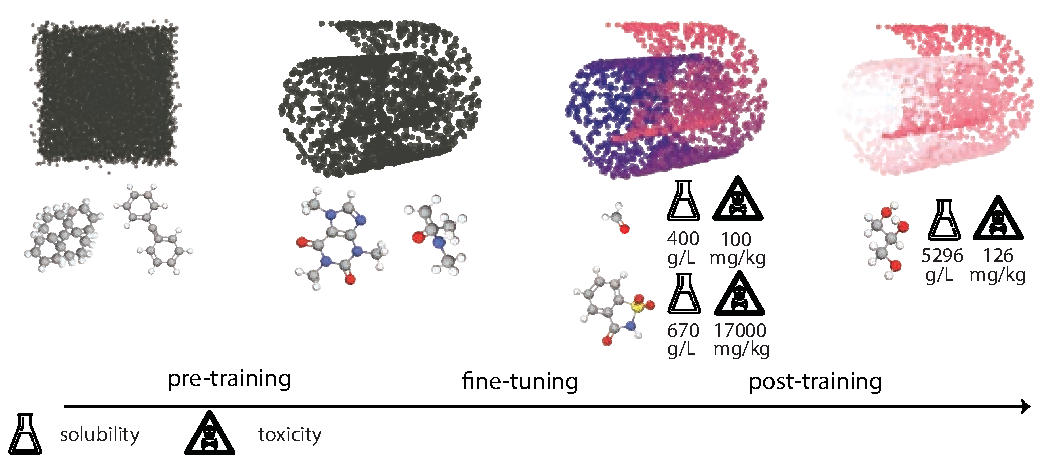
\includegraphics[width=1\textwidth]{figures/rescaled_figures/chemrev_figure4.pdf}
    \caption{\textbf{General training workflow through the lens of molecular science}. The figure illustrates the progression from pre-training through fine-tuning to post-training stages.  \textbf{(1) Pre-training:} The model learns the underlying data distribution from a vast, unlabeled dataset. This is visualized as transforming an unstructured representation space (left, square cloud) into a structured manifold (the Swiss roll). At this stage, the model has learned the \enquote{shape} of the data: the fundamental rules that make a molecule chemically valid. However, the representations are not yet specialized for any task. 
    \textbf{(2) Fine-tuning:} The model is trained on specific, labeled tasks, such as predicting solubility (flask icon) and toxicity (skull icon). This process \enquote{colors} the manifold, adjusting the learned representations so that their position now also correlates with specific properties (e.g., blue for one property profile, red for another). 
    \textbf{(3) Post-training Alignment:} The model's behavior is biased towards desired outcomes. This is visualized as preferentially sampling from a specific region of the colored manifold, such as generating molecules predicted to have high solubility and low toxicity (right, the brighter red region).}
    \label{fig:training_workflow}
\end{figure}


 Pre-training a model is teaching it to recognize this pattern. 
 By observing millions of valid examples, the model learns the \enquote{grammar} of chemistry---the principles that make a molecule physically plausible. 
 A model that has successfully learned the distribution can distinguish a valid structure from noise and can even generate new, chemically sensible examples, much like someone who has learned the rules of a language can form new, grammatically correct sentences.  

A model does not learn the data distribution by storing an explicit formula. Instead, during pre-training (see \Cref{sec:pretraining} for more details), it learns to create an internal representation---an embedding (see \Cref{sec:embeddings}).
The training process guides the model to map inputs to these embeddings in a structured manner, forming a high-dimensional space, where representations of similar, valid inputs are clustered together.


The second step is post-training, also called fine-tuning, in which the model is adapted to learn task-specific labels and capabilities, essentially \enquote{coloring} the learned structure with domain-specific knowledge. 
Crucially, fine-tuning does not discard the learned distribution but refines it. 
As shown in \Cref{fig:training_workflow}, the fundamental shape of the manifold (the Swiss roll) is preserved. 
The \enquote{coloring} process corresponds to adjusting the internal representations so they now also encode task-specific properties. 
For example, the model learns to map molecules with high solubility to one region of the manifold (e.g., the red area) and those with high toxicity to another. 
The representation of each molecule is thus enriched, now containing information not just about its structural validity but also about its properties.

Finally, techniques such as \gls{rl} are used to align the model's outputs with preferred choices. 
This step further refines the learned distribution by biasing the model's sampling behavior to favor specific modes of the distribution. 
In terms of the representation space, the model learns to prioritize generating or paying attention to points in desirable regions. As depicted in the post-training panel of \Cref{fig:training_workflow}, this biases the output towards a specific section of the colored manifold---in this case, perhaps molecules with high solubility (the brighter pink region).



\subsection{Pre-training: Learning the Shape of Data}
\label{sec:pretraining}

Pre-training establishes the foundational knowledge and capabilities of the model. 
During pre-training, the model learns general patterns, relationships, and structures from massive datasets (often trillions of tokens, see \Cref{fig:scale_of_data}). 
The model learns to map input to internal representations or features through so-called \gls{ssl} objectives like reconstructing corrupted inputs (predicting masked tokens, or predicting future sequences, see \Cref{sec:ssl}). 

This large-scale pre-training allows models to capture rich representations of the statistical distributions inherent to the data.  These learned distributions capture the fundamental patterns and structure of the domain (scientific language grammar, physical and chemical principles that govern materials). \Cref{fig:training_workflow} illustrates the distribution captured, from an uninstructed manifold prior to pre-training (if you randomly pick from this manifold, you get noise or non-physical molecules) to a structured manifold, where if you sample from this distribution (the black Swiss roll) you get a valid molecule.
For example, the model might learn commonly occurring structures, scientific notations, and scientific terms. 
Furthermore, it might construct hierarchical relationships between these concepts, such as those between chemical compounds, elements, and their properties.  
This distributional learning empowers the model to make predictions about new examples by understanding their relation to the learned patterns. Crucially, this ability stems from the development of transferable features, rather than mere data memorization \autocite{brown2020language}. 

As illustrated by the Swiss roll in \Cref{fig:training_workflow}, the pre-training process creates a structured manifold where invalid inputs are mapped far away. Therefore, learning high-quality representations is the concrete computational method for capturing the abstract statistical distribution of the data; the structure of this representation space is the model's learned approximation of the data's true shape.

\subsubsection{Self-Supervision} \label{sec:ssl}

\glspl{ssl} allows models to learn from unlabeled data by generating \enquote{pseudo-labels} from the data's structure. 
The original, unlabeled data serves as its own \enquote{ground truth}. 
This differs significantly from supervised learning, a traditional method where models are trained using labeled datasets. 
In supervised learning, each piece of data is explicitly tagged with the correct output, which the model then learns to predict. 
Such manual labeling is often an expensive, time-consuming, and domain-specific process. 
\glspl{ssl} has emerged as a particularly effective strategy for pre-training \glspl{llm}, since natural-language corpora are abundant but rarely annotated. 
Proxy strategies have then been applied to other types of model architectures as well. 
The ability to extract structure from data \textit{without labels} is a key enabler for foundation models and underpins the pre-training phase.

\subsubsection{Families of Self-Supervised Learning}

\gls{ssl} encompasses a variety of approaches. While distinct methods exist, they can be grouped into broader families based on their underlying principles. \Cref{fig:types_ssl} illustrates the two main families: generative and contrastive, along with example pretext tasks for each.

\begin{figure}[H]
    \centering
    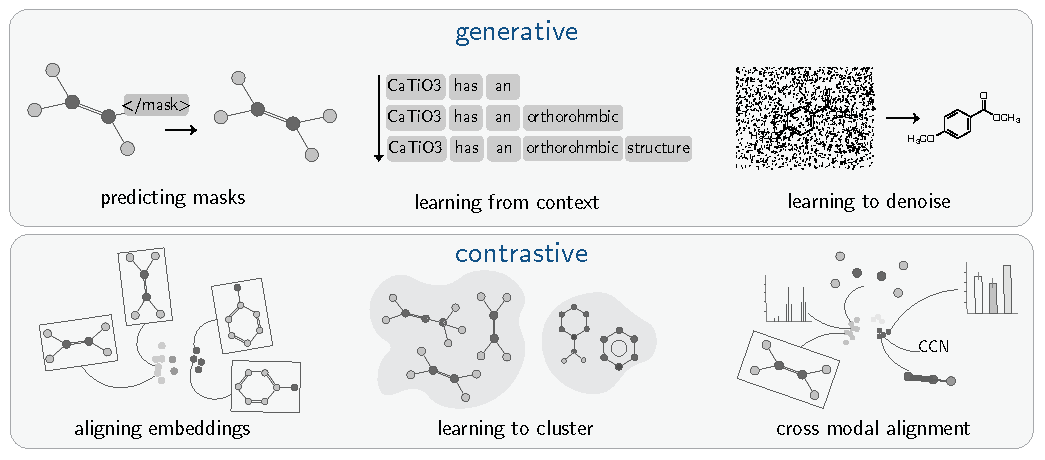
\includegraphics[width=1\textwidth]{figures/rescaled_figures/chemrev_figure5.pdf}
    \caption{\textbf{Main families in \glspl{ssl}}. The figure illustrates the two primary approaches to \gls{ssl}, each using different strategies to generate pseudo-labels from the data itself.
    \textbf{Generative Methods (Top Panel):} This family focuses on reconstruction and prediction. The model learns representations by generating missing information. Examples shown correspond to the pretext tasks discussed in the text: (1) \textit{Predicting masks} in a graph, analogous to masked modeling (more details in \Cref{sec:masked_modeling}); (2) \textit{Learning from context}, which is the basis for next token prediction (more details in \Cref{sec:next_token_prediction}); and (3) \textit{Learning to denoise}, where the model reconstructs a clean input from a corrupted version. (see \Cref{sec:denoising})
    \textbf{Contrastive Learning (Bottom Panel):} This family learns by comparing samples. The model is trained to pull representations of similar samples together while pushing dissimilar ones apart. Examples include: (1) \textit{Aligning embeddings} from different augmentations of the same molecule, a core idea in Instance Discrimination (more details in \Cref{sec:instance_discrimination}); (2) \textit{Learning to cluster} similar molecules together, as in Clustering-based Contrastive Learning (see \Cref{sec:clustering_cl}); and (3) \textit{Cross-modal alignment}, where representations from different data types (e.g., a molecule's graph and its spectral properties) are learned jointly. (see \Cref{sec:contrastive_learning} )}
    \label{fig:types_ssl}
\end{figure}

\subsubsection{Generative Methods}

This family of methods focuses on learning representations by reconstructing or predicting parts of the input data from other observed parts. 
The model learns the underlying data distribution by learning to re-generate the missing information. 
Examples shown in \Cref{fig:types_ssl} include predicting masked portions of a graph, learning from surrounding text context, and learning to denoise an image.

\label{sec:masked_modeling}
\paragraph{Masked Modeling}  In this method, portions of the input data are intentionally obscured or \enquote{masked}. The model's primary objective is then to reconstruct these hidden segments accurately. \autocite{devlin2018bert0} 
This process can be conceptualized as a \enquote{fill-in-the-blanks} task, compelling the model to infer missing information from its context. This enables the model to develop a deep understanding of contextual dependencies of data's structure and semantics without requiring explicit human-labeled annotations. For chemical data, this could involve masking and predicting tokens in \glspl{smiles}/\glspl{selfies} strings \autocite{chithrananda2020chemberta, zhang2025scientific} (i.e., hiding atoms and training the model to guess what is missing), omitting atom or bond types in molecular graphs \autocite{mahmood2021masked,wang2022molecular, reiser2022graph}, removing atomic coordinates in 3D structures, or masking sites within a crystal lattice.



\paragraph{Next Token Prediction} 
\label{sec:next_token_prediction}
Many forms of data, such as text, can be represented as sequences of tokens. 
One of the most powerful \gls{ssl} tasks for such sequential data is next-token prediction.
Here, the core objective is for a model to anticipate and generate the subsequent token in a given sequence, based on the contextual information provided by preceding tokens. 
Because text unfolds naturally in a sequence, it offers the reference information the model needs in order to learn. This approach has been applied to chemical and material representations by treating molecular string representations (\glspl{smiles}, \glspl{selfies}, etc.) or material representations as sequences \autocite{adilov2021generative, wang2023cmolgpt, schwaller2019molecular, alampara2024mattext}. 
During training, the model constantly adjusts itself to maximize the likelihood (trying to make good predictions more probable and bad predictions less probable). In this context, likelihood refers to the probability of observing the actual subsequent token given the preceding tokens in the sequence . This is accomplished by making each prediction based on the preceding input, which establishes the conditional context (see \Cref{eq:nexttoken}).


\begin{tcolorbox}[
    title= Cross-Entropy Loss,
    breakable,
    enhanced,
    colback=white,
    colframe=black!30,
    colbacktitle=black!10,
    coltitle=black,
    fonttitle=\bfseries,
    boxrule=0.5mm,
    left=2mm,
    right=2mm,
    top=4mm,
    bottom=4mm,
    middle=10mm
]
\label{eq:nexttoken}
\begin{center}
\begin{minipage}{0.9\linewidth}
\begin{equation}
\mathcal{L} = 
-\mathbb{E} \left[ \sum_{t=1}^{T} 
\log P(\eqnmarkbox[PositiveColor]{pred}{x_t} | \eqnmarkbox[NegativeColor]{context}{x_{<t}})
\right]
\label{eq:cross_entropy}
\end{equation}
\annotate[yshift=1.1em]{above}{pred}{Prediction term}
\annotate[yshift=-1.3em]{below}{context}{Conditional context}
\begin{tikzpicture}[overlay, remember picture]
\end{tikzpicture}
\end{minipage}
\end{center}
\tcblower
\begin{itemize}
\item \textbf{Prediction Term} ({\color{PositiveColor}Blue}): The target token $x_t$ that the model is trying to predict at each position.
\item \textbf{Context Tokens} ({\color{NegativeColor}Maroon}): The set of tokens $x_{\text{context}}$ the model uses to make its prediction. The definition of this context depends on the SSL task:
            \begin{itemize}
                \item \textit{For Masked Modeling:} The context is all unmasked tokens in the sequence.
                \item \textit{For Next-Token Prediction:} The context is the preceding tokens ($x_{<t}$).     
            \end{itemize}
%\item \textbf{Conditional Context} ({\color{NegativeColor}Maroon}): The previous tokens $x_{<t}$ that the model conditions on to predict the next token.
\item \textbf{Summation} $\sum_{t=1}^{T}$: The loss is calculated across all token positions in the sequence of length $T$.
\item \textbf{The Logarithm's Role}: The negative logarithm ($\log P$) heavily penalizes highly confident wrong answers (low $P$, high loss) and lightly rewards confident correct answers (high $P$, low loss).
\item \textbf{Overall Loss Structure}: Cross-entropy loss that encourages the model to assign high probability to the correct next token at each position, given all previous tokens.
\end{itemize}
\end{tcolorbox}

\paragraph{Denoising}
\label{sec:denoising}
Denoising \glspl{ssl} works by intentionally adding noise to the inputs and then training models to reconstruct the original data. In this context, the original, uncorrupted data implicitly serves as the label or target for the training process.  In this paradigm, we begin with a clean input, which we can call $x$. We then apply a random corruption process to create a noisy version, $\tilde{x}$. 
The model is then trained to reverse this damage and recover the original, clean $x$ from the corrupted $\tilde{x}$. 
This process is formally expressed as sampling a corrupted input $\tilde{x}\sim q(\tilde{x}|x)$ and optimizing the network to predict $x$. \autocite{vincent2010stacked}
By learning to recover the clean input, the model is compelled to develop robust representations that are inherently invariant to the types of noise it encounters during training.  
This directly forces the model to learn the underlying data distribution.  
To distinguish the original signal from the artificial noise, the model must learn the features of high-probability samples within that distribution. 
For example, to successfully \enquote{denoise} a molecule, it must implicitly understand the rules of chemical plausibility---the very patterns that separate valid structures from random noise.  
While popular in images \autocite{vincent2008extracting, bengio2013generalized}, denoising objectives have also been applied to graph representations of molecules \autocite{wang2023denoise, ni2024pre}. 
For instance, one can randomly perturb atoms or edges in a molecular graph and train a graph neural network to predict the original attributes. 


\subsubsection{Contrastive Learning}
\label{sec:contrastive_learning}
The other main family of \gls{ssl} techniques is contrastive learning. The objective is to train models to understand data by distinguishing between similar and dissimilar samples. 
This is achieved by learning an embedding space where representations of samples that are alike in their core chemical properties or identity are pulled closer together. In contrast, representations of samples that are fundamentally different are pushed further apart. \autocite{hadsell2006dimensionality}

This process creates meaningful clusters for related concepts while enforcing separation between unrelated ones. 
In effect, the model learns the data's underlying distribution by defining the distance between its points. 
The resulting internal representations become highly robust because they are trained for invariance; the model learns to focus on essential, identity-defining features while disregarding irrelevant variations. 
This process, often referred to as embedding alignment, ensures that the representations capture the core characteristics shared among similar samples.

There are many contrastive learning approaches with variations in loss functions. A key design choice in contrastive learning is whether to compute the contrastive loss on an instance basis or a cluster basis.


\paragraph{Instance Discrimination}
\label{sec:instance_discrimination}
Instance Discrimination is arguably the most dominant paradigm in recent contrastive learning.
Each instance (sample) in the dataset is treated as its own distinct class.  
This is typically achieved using contrastive loss functions like \modelname{InfoNCE} see \Cref{eq:infonce}. \autocite{oord2018representation} As detailed in \Cref{eq:infonce}, the loss function is formulated as a categorical cross-entropy loss where the task is to classify the positive sample correctly among a set of negatives plus the positive itself.

In materials and chemistry, this can involve aligning the textual representation of a structure with a graphical representation, image, or other visual method to represent a molecule. 
The model could also learn from augmentations of a structure, such as being given several valid \gls{smiles} strings that all describe the identical molecule. 
Furthermore, this approach can involve contrasting variations of a crystal structure against entirely different molecules or materials, enabling the model to grasp the subtle similarities and stark differences between them.



\begin{tcolorbox}[
    title=InfoNCE Loss Function,
    breakable,
    enhanced,
    colback=white,
    colframe=black!30,
    colbacktitle=black!10,
    coltitle=black,
    fonttitle=\bfseries,
    boxrule=0.5mm,
    left=2mm,
    right=2mm,
    top=4mm,
    bottom=4mm,
    middle=10mm
]

\begin{center}
\begin{minipage}{0.9\linewidth}

\begin{equation}
\label{eq:infonce}
%\mathcal{L}_{\text{InfoNCE}}
\hspace*{-2em}
\mathcal{L} = 
%\hspace*{-3em}
-\mathbb{E} \left[ \log \frac{
\eqnmarkbox[PositiveColor]{pos}{\exp({\text{sim}(f(\mathbf{x}_i), f(\mathbf{x}_i^+))/\tikzmarknode{tau1}{\tau}})}
}{
\eqnmarkbox[PositiveColor]{pos2}{\exp({\text{sim}(f(\mathbf{x}_i), f(\mathbf{x}_i^+))/\tau})} + 
\eqnmarkbox[NegativeColor]{neg}{\sum_{j=1}^{N} \exp({\text{sim}(f(\mathbf{x}_i), f(\mathbf{x}_j^-))/\tikzmarknode{tau2}{\tau}})}
} \right]
\end{equation}

\annotate[yshift=1.5em]{above}{pos}{Positive pair similarity}
\annotate[yshift=-1.5em]{below}{neg}{Negative pairs similarity}
\annotate[yshift=1em, xshift=1em]{right}{tau1}{Temperature parameter}

\begin{tikzpicture}[overlay, remember picture]
\end{tikzpicture}
\end{minipage}
\end{center}

\tcblower


\begin{itemize}
\item \textbf{Positive Pair Term} ({\color{PositiveColor}Blue}): Measures similarity between an anchor sample $\mathbf{x}_i$ and its positive pair $\mathbf{x}_i^+$ (e.g., different view of the same molecule).

\item \textbf{Negative Pairs Term} ({\color{NegativeColor}Maroon}): Sum of similarities between anchor sample $\mathbf{x}_i$ and all negative pairs $\mathbf{x}_j^-$ (e.g., different molecules).

\item \textbf{Temperature Parameter} $\boldsymbol{\tau}$ %({\color{TemperatureColor}})%
: Controls the sharpness of the distribution. Lower values make the model more sensitive to hard negatives.

\item \textbf{Overall Loss Structure} %({\color{OverallColor}Purple})%
: A negative log probability that encourages the model to maximize similarity for positive pairs while minimizing it for negative pairs.
\end{itemize}

\end{tcolorbox}


\paragraph{Clustering-based Contrastive Learning} 
\label{sec:clustering_cl}
Clustering approaches leverage the idea that similarity often translates to closeness in the feature space. Methods like \modelname{DeepCluster} \autocite{caron2018deep}  iteratively train a model. First, they group the generated features (internal representation) of a dataset into distinct sets using a common grouping algorithm, such as $k$-means clustering. Imagine you have a pile of diverse objects; $k$-means would help you sort them into a predefined number of piles based on their similarities, like color or shape. 
These assigned groups then act as \enquote{pseudo-labels}---temporary, automatically generated labels---to train the network. 
The supervised training step implicitly contrasts samples from different clusters. The clustering and training steps alternate. 
Take a dataset of molecular fingerprints as an example. A model can be trained to predict the clustering pattern of this fingerprint data, distinguishing between conformer types or perturbed structures. Thus, the model learns representations that group chemically or structurally similar fingerprints. 



\subsection{The Holy Grail of Building Good Internal Representation} 

The design of effective pretext tasks---such as specific versions of instance discrimination (identifying unique examples) or denoising (recovering original data from corrupted versions)---is perhaps the holy grail. This is precisely where deep domain expertise becomes invaluable.

The pretext tasks must be meaningful, preserving the core identity of the molecule or material while introducing sufficient diversity to challenge the model and allow it to learn robust invariances.

For instance, a suboptimal technique would be to shuffle all the atoms in the text representation of a molecule. 
This would destroy the molecule's chemical meaning, which would hinder the model's ability to learn chemically meaningful features. 
Good augmentations typically enable richer features by providing additional layers of information to learn from, such as generating different low-energy conformers or using non-canonical string representations.


\paragraph{Parallels between Generative and Contrastive Objectives}

While it might seem that generative and contrastive \glspl{ssl} methods optimize different things, their underlying goals can often be equivalent. 
A generative masked language model learns the conditional probability
(see \Cref{eq:infonce})
, aiming to assign a high probability to the correct masked token by effectively discriminating it from other vocabulary tokens. 
The \modelname{InfoNCE} loss in contrastive learning can be viewed as a log-loss for a $(K+1)$-way classification task (see \Cref{eq:infonce}). 
Here, the model learns to identify the positive pair $f(x_i^+)$ as matching $f(x_i)$ from a set including $f(x_i^+)$ and $K$ negative features $f(x_j^-)$. 
Both approaches effectively learn to select the \enquote{correct} item (a token or a positive feature) from a set of candidates based on the provided context or an anchor. 
To do so, they must effectively build strong internal representations.




\paragraph{Pre-training beyond \gls{ssl}}
Pre-training cannot be performed using \gls{ssl} on a single modality alone.  For example, in models that consider multiple input formats (multimodality, as explained in detail in \Cref{sec:multimodal_chem}), alignments between different modalities (e.g., text-image, text-graph) serve as a pre-training step.\autocite{weng2022vlm,girdhar2023imagebind0}  General-purpose force fields are commonly trained in a supervised manner on relaxation and simulation trajectories.\autocite{batatia2022mace, wood2025uma0}
Thus, the model learns a representation of connectivity patterns to energies. However, these representations also implicitly encode structural patterns (commonly observed coordination environments) and their correlations with each other and with abstract properties. 
A distinct and powerful pre-training paradigm moves away from real-world data entirely, instead training models like \modelname{TabPFN} on millions of synthetically generated datasets to become general-purpose learning algorithms. This allows them to perform in-context learning on new, small datasets in a single forward pass, often outperforming traditional methods. \autocite{hollmann2025accurate} \\

\noindent The core principle remains: \emph{learning on large datasets to build generalizable internal representations before task-specific fine-tuning.}

\subsection{Fine-Tuning: Learning the Coloring of Data}
\label{sec:fine_tuning_coloring}

While pre-training enables models to learn general structural representations of chemical data, fine-tuning refines these representations for specific downstream tasks.
If pre-training can be conceptualized as learning the \enquote{structure} of chemical knowledge, fine-tuning can be viewed as learning to \enquote{color} this structure with task-specific knowledge and capabilities (see \Cref{fig:training_workflow}). 
This specialization process transforms general-purpose internal representations into powerful task-specific predictors while retaining the foundational knowledge acquired during pre-training.

Fine-tuning adapts pre-trained model parameters through continued training on domain-specific datasets. 
This typically requires substantially less data than pre-training.  To make this process even more efficient, a common strategy is to \enquote{freeze} the majority of the model’s layers and only train a small subset of the final layers (see \Cref{sec:peft}).
Fine-tuning is particularly valuable in chemistry, where datasets are often limited in size.
Traditionally, addressing chemistry-specific problems required heavily engineered and specialized algorithms that directly incorporated chemical knowledge into model architectures.  
However, fine-tuned \glspl{llm}, for example, have shown comparable or superior performance to these specialized techniques, particularly when data is limited \autocite{jablonka2024leveraging}. 
The efficiency of fine-tuning stems from the transferability of chemical knowledge embedded during pre-training, where the model has already learned to spot patterns in molecular structure, reactivity, and chemical terminology sequences. With a large amount of data \glspl{llm} compress a lot of such sequence relationships into its weights.

\subsection{Post-Supervised Adaptation: Learning to Align and Shape Behavior} \label{sec:rl}

Pre-training and fine-tuning equip the model with a learned distribution, which represents its knowledge about what outputs are plausible or likely. 
Post-training does not erase this knowledge; instead, it biases this distribution towards preferred outcomes---such as task-specific goals. 
The new, desired behavior of the model (called the policy, $\pi$, in \gls{rl}) comes from this refined distribution.
This shift has a subtle but crucial effect on the internal representations. 

Post-training alignment workflows commonly use \gls{rl}, as the classic loss-minimization approaches---simply fine-tuning on more \enquote{correct} examples---can struggle to capture more nuanced, hard-to-label objectives\autocite{Huan2025mathLLM}; when the goal is to steer the model toward more intangible qualities, formulating loss functions and collecting a pre-labeled dataset become very challenging. 
In \gls{rl}-based alignment, the model is treated as an agent that takes actions (generates text in the case of an \gls{llm}) in a trial-and-error environment and receives a reward signal based on the actions it chooses. 
The \gls{rl} objective is to maximize this reward by changing the model's behavior. In the case of \gls{llm}, this means compelling it to generate text with the preferred properties. 
This process transforms the model into a goal-oriented one, where the goal can be to generate stable molecules, solve tasks step by step, or utilize tools, depending on the reward function.

During alignment, the foundational embeddings for basic concepts (e.g., a carbon atom) learned during pre-training remain largely intact. 
This initial state is critical; without a robust, pre-trained \gls{llm}, the \gls{rl} process would be forced to blindly explore an intractably vast space, making it highly unlikely to discover preferred sequences (that it could then reinforce).   
 
The mapping from an input to its final representation is adjusted to become \enquote{reward-aware}. For example, the representation of a molecule might now encode not just its chemical structure, but also its potential to become a high-reward final molecule (stable and soluble molecule) \autocite{narayanan2025training}. 
The representation space retains its overall shape (\Cref{fig:training_workflow}), but the model learns a new way to navigate it, guided by the reward.
\begin{tcolorbox}[
    title=Reinforcement Learning Framework for \glspl{llm},
    breakable,
    enhanced,
    colback=white,
    colframe=black!30,
    colbacktitle=black!10,
    coltitle=black,
    fonttitle=\bfseries,
    boxrule=0.5mm,
    left=2mm,
    right=2mm,
    top=6mm,
    bottom=4mm,
    middle=12mm
]
\label{eq:rl}

\begin{center}
\begin{minipage}{0.9\linewidth}
\vspace{1.5em}

\begin{equation}
\label{eq:rl_objective}
\hspace*{-1em}
\pi(a|s) = \eqnmarkbox[PolicyColor]{policy}{P_{\text{LLM}}} \left( \eqnmarkbox[ActionColor]{action}{\text{next tokens}} \mid \eqnmarkbox[StateColor]{context}{\text{context}} \right) 
\rightarrow \text{Maximize } \eqnmarkbox[RewardColor]{reward}{\mathbb{E}[R]}
\end{equation}

\vspace{1.5em}

\annotate[yshift=1.5em, xshift=-1em]{above,right}{context}{State}
\annotate[yshift=-1.5em, xshift=1em]{below,right}{action}{Action}
\annotate[yshift=1.5em]{above}{policy}{Policy (\gls{llm})}
\annotate[yshift=-1.5em]{below}{reward}{Expected Reward}

\vspace{0.5em}

\end{minipage}
\end{center}

\tcblower

\begin{itemize}
\item \textbf{State ($s$)} ({\color{StateColor}Blue}): The sequence of tokens generated so far, including the original prompt and any partial response. Represents the current context that the model uses to make decisions.

\item \textbf{Action ($a$)} ({\color{ActionColor}Maroon}): The next token that the model chooses to generate from its vocabulary. This is the discrete decision the agent makes at each step.

\item \textbf{Policy ($\pi$ or $P_{\text{LLM}}$)} ({\color{PolicyColor}Red}): The \gls{llm} itself, whose parameters define the probability distribution over possible following tokens given the current state. This is what gets optimized during training.

\item \textbf{Reward ($R$)} ({\color{RewardColor}Peach}): A numerical score assigned to complete generated sequences, measuring how well the output achieves the desired goal. Used only during training to guide parameter updates.

\item \textbf{Expectation ($\mathbb{E}$)} ({\color{RewardColor}Peach}): The average cumulative reward, calculated over many possible sequences that could be generated by the current policy. 

\item \textbf{Training Objective}: Adjust the model's parameters to maximize the expected cumulative reward ($\mathbb{E}[R]$) over complete sequences, enabling the generation of high-quality outputs.
\end{itemize}

\end{tcolorbox}

\paragraph{The Challenge of Reward Design}
A critical factor for the success of this framework is the design of the reward function. The training process is most stable and effective when rewards are \textit{verifiable} and based on objective, computable metrics. 
In contrast, training with \textit{sparse} rewards (where feedback is infrequent) or \textit{fuzzy} signals (where the goal is subjective or ill-defined) makes the credit assignment problem significantly more difficult. 
This is a central challenge in aligning models with complex human preferences, as crafting precise reward functions that capture the full nuance of a desired behavior remains an active area of research \autocite{ouyang2022training}.


\paragraph{The \gls{llm} as a Policy}
When using a \gls{llm} as the agent in \gls{rl}, the policy (see \Cref{eq:rl_objective}) is the \gls{llm} itself. 
Consider teaching a model to design multi-step synthetic routes for pharmaceutical compounds, using a retrosynthetic strategy. 
The \textbf{state} ($s$) represents the synthetic plan generated so far. Initially, the state consists of just the target molecule but evolves to include each proposed step in the route. Each \textbf{action} ($a$) is the next retrosynthetic decision---for example, which bonds to break or what reagents to use. The \gls{llm} serves as the policy ($\pi$), using its parameters to determine the probability of choosing different possible actions given the current context. 
To put it mathematically, this would be $\pi(a|s) = P_{\text{LLM}}(\text{next synthetic step}|\text{current plan})$ (see \Cref{eq:rl_objective}). 
The model leverages its chemical knowledge to identify the most promising decisions. 
The \textbf{reward} ($R$) scores the completed retrosynthetic route based on practical criteria that could be the number of steps, predicted yield, reagent cost, etc. 
This score can directly come from the feedback of real chemists (\gls{rlhf}), or from a small model trained to predict human preference scores or pre-defined criteria.

Theoretical work in reinforcement learning has shown that the complexity of such problems scales quadratically with the size of the action space \autocite{dann2015sample}. 
At each step, the model must choose from tens of thousands of possible tokens, and the number of possible sequences (and therefore actions) grows exponentially. 
Without pre-training, this would make the learning process computationally prohibitive. Pre-training provides a strong initialization that effectively constrains the action space to reasonable chemical language and valid synthetic steps, dramatically reducing the exploration requirements (see how pre-training creates a structured manifold in \Cref{fig:training_workflow}).

Recent developments have revealed that \gls{rl} training can elicit reasoning capabilities that were previously thought to require explicit programming or extensive domain-specific architectures. 
Models trained with \gls{rl} demonstrate the ability to decompose complex problems, perform backtracking when approaches fail, and engage in multi-step planning without being explicitly taught these strategies. \autocite{xu2025towards}

\paragraph{Updating the LLM Policy} 
After the model takes actions (generates a sequence of tokens), the reward it receives for the chosen actions is used to update the \glspl{llm} parameters using an \gls{rl} algorithm, such as \gls{ppo} \autocite{schulman2017proximal}.
\gls{ppo} works by encouraging the model to favor actions (outputs) that lead to higher rewards, but it also includes a mechanism to constrain how much the model's behavior can change in a single update. 
Specifically, it introduces a penalty term that discourages the \glspl{llm} policy from deviating too far from its original, pre-trained distribution. 
This ensures the model does not \enquote{forget} its foundational knowledge about language or chemistry while it is learning to pursue the reward, thus biasing the distribution rather than completely overwriting it. 
The result is a controlled shift: the model becomes more aligned without losing what it already knows.


\paragraph{Inference and Sampling from the Adapted Model}

The \gls{rl} training process permanently updates the weights of the \gls{llm}. 
When we sample from this model, we are drawing from this new, biased distribution. 
For a given context (state), the probabilities for tokens (actions) that were historically part of high-reward sequences are now intrinsically higher. 
At the same time, pathways that led to low rewards are suppressed. 
The model is now inherently more likely to generate outputs that align with the preferences and goals encoded in the reward function.

\subsection{Example Architectures} \label{sec:example_architectures}
While much effort is currently invested in building foundation models based on transformer-based \glspl{llm}, the foundation model paradigm is not limited to this model class.

In the chemical domain, where heterogeneous data such as \gls{smiles} and graphs for molecular structures prevail, the use of a diverse array of architectures is expected.
The architectures shown in \Cref{fig:architectures} are examples of foundational backbones that we discuss in the following sections.

\begin{figure}[H]
    \centering
    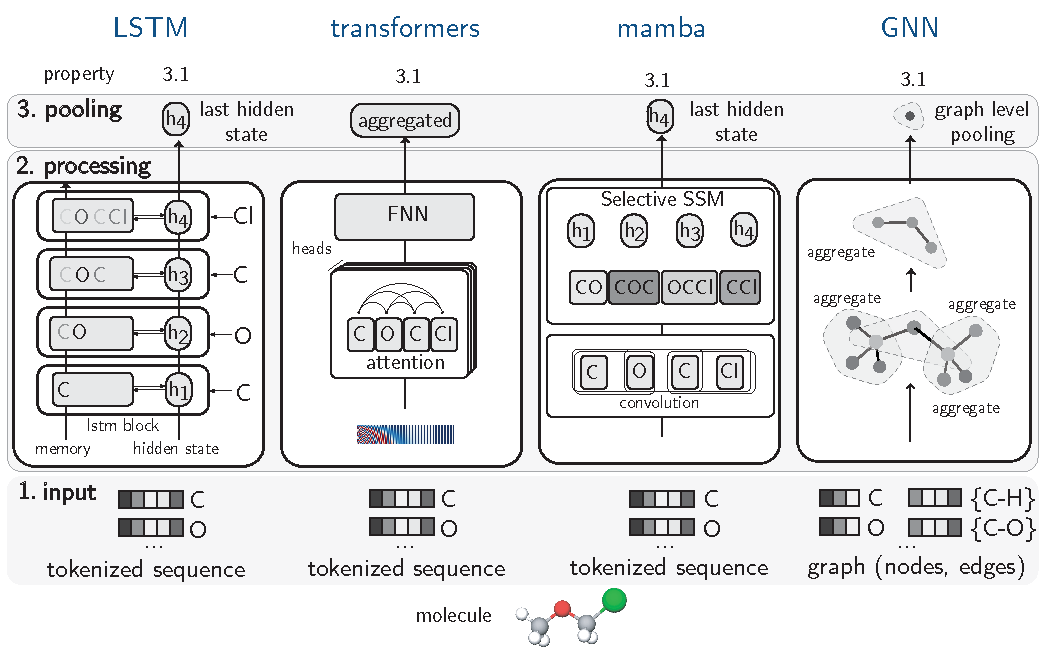
\includegraphics[width=1\textwidth]{figures/rescaled_figures/chemrev_figure6.pdf}
    \caption{\textbf{Blueprint for \glspl{gpm} architectures}. This diagram illustrates four distinct neural network architectures (\gls{lstm}, Transformer, Mamba, and \gls{gnn}), highlighting their unique approaches to input representation, information processing, and output pooling. \glspl{lstm} sequentially process tokens, accumulating information in a final hidden state with an inductive bias towards order. Transformers, conversely, use multi-head attention and positional encodings to capture global interactions simultaneously, offering minimal inductive bias but enabling rich contextual understanding. Mamba combines local convolutional processing with selective state space modeling to efficiently focus on chemically relevant parts, also typically using a final hidden state. \glspl{gnn} leverage the inherent graph structure of molecules, where atoms are nodes and bonds are edges, to model local chemical environments through message passing, followed by graph-level pooling to create a unified representation. Each approach offers unique strengths in how it captures molecular features, ranging from sequential to global, and graph-based relationships.}
    \label{fig:architectures}
\end{figure}


\paragraph{\gls{lstm}}

\gls{lstm} networks \autocite{hochreiter1997long} are well-suited for processing sequential data, such as text or time series. 
\Cref{fig:architectures} illustrates how chemical information is processed to predict \glspl{lstm}.
\begin{itemize}
    \item \textbf{Input}: Molecules are represented as tokenized sequences (e.g., \gls{smiles} strings like \enquote{COCCl}), processed one token at a time. Each token corresponds to an atom.
    \item \textbf{Processing}: Information flows sequentially through \gls{lstm} blocks where each hidden state ($h_{1}$, $h_{2}$, $h_{3}$, $h_{4}$) accumulates information about the molecule. The memory cell maintains chemical context through gating mechanisms. The inductive bias is sequential processing---assuming chemical properties emerge from analyzing tokens in order.
    \item \textbf{Pooling}: The final hidden state ($h_{4}$) captures the entire molecular information after processing the complete sequence. This last state serves as the molecular representation for the downstream task.
\end{itemize}

\glspl{lstm} process information in a strict sequence.  For the model to connect the first word to the last, that information must pass through every single step in between. The cost of \enquote{talking} across the sequence grows with the sequence length. 
Furthermore, the entire history of the sequence must be compressed into a single, fixed-size hidden state.

An \gls{xlstm} overcomes this with two key changes. \gls{xlstm} uses enhanced gates (act like filters to control what information flows) to precisely revise its memory. Second, instead of a single memory bottleneck, it uses a parallel \enquote{matrix memory}. This provides multiple \enquote{slots} to store different pieces of information at the same time. This structure allows it to process information in parallel, making it much more efficient.
\modelname{Bio-xLSTM} adapts this architecture for biological and chemical sequences, demonstrating proficiency in generative tasks and in-context learning for DNA, proteins, and small molecules.\autocite{SchmidingerSSSH25}


\paragraph{Transformer}

Transformers \autocite{vaswani2017attention} are also designed for sequential data, but are particularly powerful in capturing long-range dependencies and rich contextual relationships within sequences. 
Their core \enquote{attention mechanism} allows them to weigh the importance of different parts of the input simultaneously (quadratic computational scaling---if you double the length of the sequence, the amount of work the model needs to do quadruples). 
Effectively, they can be thought of as a fully connected graph model,\autocite{velivckovic2023everything, joshi2025transformers} where each representation of a token is connected to every other token and can impact its representation.

\begin{itemize}
    \item \textbf{Input}: Similar to \glspl{lstm}, data is tokenized and often enhanced with positional encodings (see \Cref{fig:architectures}, the tokenized sequence is added with positional information, e.g., using a sinusoidal signal---the red-blue spectrum) to maintain information about where in a sequence a token is placed (the attention mechanism itself does not preserve this information).
    \item \textbf{Processing}:  Uses attention mechanisms, where every atom/token attends to every other token simultaneously. This enables the capture of long-range interactions between distant elements of the sequence, regardless of their sequential distance. The \gls{fnn} transforms these attention-weighted representations.  To get a more robust and comprehensive understanding of the relationships within a sequence, models don't just rely on a single way of \enquote{paying attention}.  Instead, they employ multiple independent \enquote{attention heads} known as multi-head attention.
    \item \textbf{Pooling}:  Uses an aggregated representation or special token that combines information from all tokens, enabling global molecular property prediction.
\end{itemize}

\paragraph{Mamba}
Mamba\autocite{gu2023mamba0} is designed to be highly efficient (linear computational scaling) and effective at modeling very long sequences, offering a potentially more scalable alternative to Transformers for certain sequential tasks (for example, modelling very long protein sequences or polymer chains, while retaining strong performance in capturing dependencies.

\begin{itemize}
    \item \textbf{Input}:  Sequences similar to \gls{lstm}.
    \item \textbf{Processing}:  First applies convolution to capture local contexts, creating representations that incorporate neighboring information. These contextualized tokens are then processed through a \gls{ssm}. An \gls{ssm} is a type of sequence model that efficiently captures and summarizes long-range dependencies by tracking an evolving internal \enquote{state} (evolving representation of all the relevant information) based on inputs. This \gls{ssm} dynamically focuses on relevant parts. The inductive bias combines local patterns (through convolution) with efficient selective attention for handling long-range dependencies.
    \item \textbf{Pooling}:  Uses the final hidden state ($h_{4}$) similar to \gls{lstm}, but this state contains selectively processed information that more efficiently captures important features.
\end{itemize}
This architectural approach has been successfully applied to chemical foundation models, demonstrating \gls{sota} results in tasks like molecular property prediction and generation while maintaining fast inference on a large dataset of \gls{smiles} samples.\autocite{soares2025mamba-based} 



\paragraph{\gls{gnn}}
\gls{gnn} is an architecture that complements graph representations (see the section discussing graph-based representation \Cref{sec:common_representations}). Molecules are represented as graphs, where atoms are nodes and bonds are edges. \glspl{gnn} operate on these graphs by processing node and edge representations. Based on how the nodes are connected through edges, the information in these representations is updated multiple times. This procedure is called message passing (see \Cref{fig:architectures}). Information from neighbors is aggregated, and this aggregation occurs for all nodes and sometimes also for edges.

\begin{itemize}
    \item \textbf{Input}: Graphs, which are collections of nodes (e.g., atoms) and edges (e.g., bonds).
    \item \textbf{Processing}: Uses message passing through multiple aggregation steps (message would be the information in node or edge at the current stage, and aggregation can be different types of operations like adding information, taking mean, etc, depending on the architecture choice). Each node updates its representation based on messages from its bonded neighbors. The inductive bias is the graph structure itself, which naturally aligns with chemical bonding patterns.
    \item \textbf{Pooling}: Graph-level pooling (e.g., taking the mean of all node representations) aggregates information from all atoms and bonds to create a unified molecular representation, respecting the molecular graph structure.
\end{itemize}

\noindent These architectures cannot solve all problems equally well because they are tailored to different data structures. 
\gls{lstm} and Mamba inherently excel at processing sequential data; Transformers need to learn the structure, Transformers are powerful at capturing global relationships across the entire input,
whereas \glspl{gnn} are designed for graph-structured information. 
Forcing one type to handle data optimally it was not intended for, often leads to suboptimal performance, inefficiency, or requires extensive, task-specific adaptations that dilute its \enquote{general-purpose} nature.\autocite{alampara2024mattext}


\subsection{Multimodality}

Multimodal capabilities enable systems to process and understand multiple types of data simultaneously. 
Unlike traditional unimodal models, which work with a single data type (e.g., text-only or image-only), multimodal models can integrate and reason across different modalities, such as text, images, molecular structures, and spectroscopic data.

The core principle behind multimodal models lies in learning shared representations across different data types.  The challenge of creating this shared representation can be addressed through several architectural strategies, each with a different approach to learning the joint distribution of multimodal data. One dominant strategy is joint embedding alignment, where separate, specialized encoders are used for each modality (e.g., a \gls{gnn} for molecular structures and a Transformer for text). These encoders independently map their respective inputs into their own high-dimensional vector spaces. The key learning objective, often driven by contrastive learning (see \Cref{sec:contrastive_learning}), is to align these separate spaces. 


Another common approach is input-level fusion, where different data types are tokenized into a common format and fed into a single, unified architecture. 
For instance, a molecular structure might be converted into a \gls{smiles} string, an image into a sequence of patches, and text into its standard tokens. These disparate token sequences are then concatenated and processed by a single large model, typically a Transformer. 
This architecture allows the model's attention mechanism to learn correlations between modalities at a fundamental level directly---an image patch can \enquote{attend} to a word in the description, for instance. 
A more recent and highly efficient variant is adapter-based integration, where a powerful, pre-trained unimodal model (models that take a single type of representation) (like an \gls{llm}) is frozen, and a small \enquote{adapter network} (see discussion about adapter in \Cref{sec:model_adaptation}) is trained to project the embeddings from a secondary modality (e.g., a molecule) into the \gls{llm}'s existing latent space. 
This adapter effectively learns to translate the new data type into the \gls{llm}'s native \enquote{language}, leveraging the \gls{llm}'s vast pre-existing knowledge without the need for complete re-training. 
For instance, a model might learn that the textual description \enquote{benzene ring} corresponds to a specific visual pattern in molecular diagrams and produces characteristic peaks in \gls{nmr} spectroscopy. 
This cross-modal understanding enables more comprehensive and contextually rich analysis than any single modality alone could provide.

\subsubsection{Multimodal Integration in Chemistry}\label{sec:multimodal_chem}

A molecule’s \gls{smiles} string alone might not reveal its 3-D conformational preferences. 
A spectrum alone could suggest many different molecular structures. 
However, coupling these modalities with textual knowledge (e.g., \enquote{the sample was prepared by X method}) could narrow down possibilities. 
Multimodal models have the potential to emulate a human expert who simultaneously considers spectral patterns, chemical rules, and prior knowledge to deduce a structure. 
Another motivation is to create generalist \gls{ai} models. 
Instead of having multiple independent models---one for spectral analysis, another for molecule property prediction, and another for text mining---a single model could handle diverse tasks by understanding multiple data types.
In this way, a researcher can ask a question in natural language, provide a molecule (in the form of a structure file or image) as context, and receive a helpful answer that leverages both structural and textual knowledge.

\modelname{MolT5} \autocite{edwards2022translation} adapted the \modelname{T5} transformer for chemical language by training on scientific text and \gls{smiles} strings, using a masking objective to reconstruct masked segments. 
This approach treats \gls{smiles} as a \enquote{language}, enabling \modelname{MolT5}  to generate both valid molecules and fluent text. 
Similarly, \modelname{Galactica} \autocite{taylor2022galactica}, an \gls{llm}, also incorporated \gls{smiles} into its training. Later, the \modelname{MolXPT}\autocite{liu2023molxpt0} model used \enquote{paired} examples (\gls{smiles} and textual description) by replacing chemical names in scientific texts with their corresponding \gls{smiles} strings and description. 
This pre-training approach enables \modelname{MolXPT} to learn the context of molecules within text and achieve zero-shot text-to-molecule generation (see \Cref{sec:mol_generation} for more details on this application).

Contrastive learning emerged as an alternative, aligning separate text and molecule encoders in a shared embedding space. 
The principle of learning here is the same as that explained in \Cref{{sec:contrastive_learning}}. \modelname{MoleculeSTM} \autocite{Liu2023multi0modal} aligns separate text and molecule encoders in a shared space using paired data. 
This dual-encoder approach enables tasks such as retrieving molecules from text queries and shows strong zero-shot generalization for chemical concepts.  
Another notable study is \modelname{CLOOME} \autocite{sanchez2023cloome}, which used contrastive learning to embed bioimaging data (microscopy images of cell assays) and chemical structures of small molecules into a shared space. 
Multimodal learning also enables the determination of molecular structure from spectroscopic data. 
Models trained on large datasets of simulated spectra \autocite{alberts2024unraveling}, which combine multiple spectral inputs, could accurately translate spectra into molecular structures. \autocite{chacko2024spectro,mirza2024elucidating}


Beyond just prediction, some multimodal models aim for cross-modal generation, creating one type of data from another (e.g., generating an \gls{ir} spectrum from a molecular structure). \textcite{takeda2023multi} developed a multimodal foundation model for materials design, integrating \gls{selfies} strings, \gls{dft} properties, and optical absorption spectra. 
Their approach involves encoding each type of data separately into a shared, compressed representation space. 
Then, a network learns to combine these compressed representations to understand the connections between them. 
This pre-training on a big dataset of samples enables both combined representations (joint embeddings summarizing all modalities) and cross-modal generation, allowing tasks like predicting a spectrum from a molecule or generating a molecule from desired properties, effectively learning the relationships between structure, spectra, and quantum properties.

Their approach involves encoding each type of data (like molecular structure or properties) separately into a shared, compressed representation. 
Then, a network learns to combine these compressed representations to understand the connections between them. 

A more recent approach is the integration of molecular encoders with pre-trained \glspl{llm}. 
Models like \modelname{InstructMol} \autocite{cao2023instructmol0} and \modelname{ChemVLM} \autocite{li2024seeing} use an \enquote{adapter} (see discussion about \modelname{LoRa} in \Cref{sec:model_adaptation}) to project molecular information into the \gls{llm}'s existing knowledge space. 
This two-stage process first projects molecule representations into the \gls{llm}'s token space through pre-training on molecule-description pairs. 
Subsequently, instruction tuning on diverse chemistry tasks (e.g., \gls{qa}, reaction reasoning) enables the \gls{llm} to leverage molecular inputs, significantly enhancing its performance on chemistry-specific problems.


The latest generation of foundation models is often natively multimodal, designed from the ground up to process text, images, and other data types seamlessly. 
Natively multimodal systems are characterized by a single, unified neural network trained end-to-end on a diverse range of data modalities. 
This approach contrasts with previous methods that would stitch together separate models for each data type, enabling a more seamless and nuanced understanding of context and relationships across different informational forms. 
In the scientific domain, natively multimodal systems are still being explored. However, evaluations suggest that these models are not yet robust for solving complex scientific research tasks.\autocite{alampara2024probing}


\subsection{Optimizations}

As \glspl{gpm} continue to grow in size and complexity, optimization techniques become critical for making these models practically deployable while maintaining their accuracy. 
This section discusses three key optimization approaches that have particular promise for chemistry foundation models: \gls{moe} architectures for efficient scaling, quantization, and mixed precision for memory and computational efficiency, and knowledge distillation for creating specialized, lightweight models.


\subsubsection{Mixture-of-Experts} \label{sec:arch-moes}
\gls{moe} is a neural network architecture that uses multiple specialized \enquote{expert} networks instead of one single, monolithic model. The core idea is to divide the vast problem space---the embedding space of all possible inputs---into more manageable, homogeneous regions. A region is considered \enquote{homogeneous} not because all inputs within it are identical, but because they share similar characteristics and can be processed using a consistent set of rules. For instance, in a chemistry model, one expert might specialize in organic molecules, while another focuses on inorganic crystals; each expert sees a more consistent, or homogeneous, set of problems. This division of labor is managed by a gating network, which acts like a smart dispatcher. This gating network is itself a small neural network, often referred to as a trainable router, because it learns during training how best to route the data to the most appropriate expert, thereby improving its decisions over time.
\gls{moe} models achieve efficiency through selectively activating only the specific experts needed for a given task, rather than activating the entire neural network for every task. Modern transformer models using \gls{moe} layers can scale to billions of parameters while maintaining manageable computational costs, as demonstrated by models like \modelname{Mixtral-8x7B}, which uses eight experts with sparsity.

\textcite{shazeer2017outrageously} demonstrated that using a sparsely-gated \gls{moe} layer can expand a network’s capacity (by over 1000 times) with only minor increases in computation. In this architecture, each expert is typically a \gls{fnn}, and a trainable router determines which tokens are sent to which experts, allowing only a subset of the total parameters to be active for any given input. 
 
An \gls{llm} for science with \gls{moe} architecture (\modelname{SciDFM} \autocite{sun2024scidfm}) shows that the results of expert selection vary with data from different disciplines, i.e., activating distinct experts for chemistry vs.\ other disciplines. They consist of multiple \enquote{expert} subnetworks, each potentially specializing in different facets of chemical knowledge or types of chemical tasks. A routing mechanism directs inputs to the most relevant expert(s). This allows the foundation model to be more adaptable and perform across the broad chemical landscape.  The \gls{moe} concept has also been adapted for physical simulations. The \modelname{UMA} family employs a \gls{moe} architecture with linear experts to build accurate yet computationally efficient interatomic potentials \autocite{wood2025uma0}. This approach builds route based on  global system properties (e.g., elemental composition, charge, spin) rather than per-token.


Extending this concept, a recent multi-view \gls{moe} model (\modelname{Mol-MVMoE} \autocite{shirasuna2024multi}) treats entire, distinct chemical models as individual \enquote{experts}. Rather than routing tokens within one large model, a gating network learns to create a combined molecular representation by dynamically weighting the embeddings from each expert model. This method showed strong performance on \modelname{MoleculeNet}, a widely used benchmark suite for molecular property prediction, outperforming competitors on 9 of 11 tasks.


Training \gls{moe} models can be a complex process. The gating mechanism must be carefully learned to balance expert usage and instability, or some experts may end up underutilized (most of the data would be processed by a subset of networks). \autocite {fedus2022switch} For chemistry tasks, an additional challenge is to ensure that each expert has access to sufficient relevant chemical data to specialize. If the data is sparse, some experts may not learn meaningful functions. Despite these hurdles, \glspl{moe} remain a promising optimization strategy to handle the breadth of chemical space.



\subsubsection{Quantization and Mixed Precision}
\label{sec:quantization}
Quantization is a technique for making models more computationally efficient by reducing their numerical precision. 
In experimental science, precision often relates to the number of significant figures in a measurement; a highly precise value, such as $3.14159$, carries more information than a rounded one, like $3.14$. 
Similarly, a model's knowledge is stored in its weights, which are organized into large matrices of numbers. Standard models typically use high-precision formats, such as 32-bit floating-point, which can represent a wide range of numbers with many decimal places to store weights. During inference, these weight matrices are multiplied by the input data to produce a prediction. Quantization involves converting these numbers into a lower-precision format, such as 8-bit integers, which are whole numbers with a much smaller range. This process is similar to rounding down your experimental data---it simplifies the numbers, uses less memory, and allows calculations to run much faster.

 
\textcite{dettmers2022gpt3} introduced an 8-bit inference approach (\texttt{LLM.int8}) enabling models as large as \modelname{GPT-3} (175B parameters) to run with no loss in predictive performance (less than $50\%$ GPU-memory usage).  
A key insight in this paper is that while most numbers in a model can be safely rounded, a few \enquote{outlier} values with large magnitudes are critical for performance. 

A different, yet related, strategy is mixed-precision quantization.\autocite{micikevicius2017mixed} Instead of applying a single precision format (like 8-bit) across the entire model, this approach uses a mix of different precisions for different parts of the network. The guiding principle is that some layers of the model might be more sensitive to rounding errors than others.


Many chemistry applications, particularly in automated laboratory setups, require deployment on edge devices---local computing hardware, such as the controllers for robotic arms or the onboard computers in analytical instruments---or cloud platforms with limited computational resources. Quantization can be a valuable optimization tool for reducing computational burden while increasing inference speed, which is crucial for real-time applications.


\subsubsection{Parameter-Efficient Tuning}
\label{sec:peft}

While full fine-tuning is computationally expensive, memory-intensive, and results in a complete, multi-gigabyte copy of the model for every new task. 
\gls{peft} methods offer a solution to this problem by freezing the vast majority of the trained model's weights and only training a very small number of new parameters. This is conceptually similar to attaching a small, specialized probe to a large, complex analytical instrument; you adapt its function for a new task without re-engineering the entire machine.

A prominent and widely used \gls{peft} technique is \gls{lora}.\autocite{hu2022lora}  
The key insight of \gls{lora} is that the change needed to adapt a pre-trained weight matrix for a new task can be approximated effectively using much smaller matrices. \gls{lora} freezes the original model weights and introduces small trainable rank-decomposition matrices into each transformer layer, significantly reducing the number of trainable parameters. 
Because these new matrices contain far fewer parameters—often less than 0.1\% of the original model—the computational and memory requirements for training are drastically reduced.
 
These optimization strategies can be combined with quantization (see \Cref{sec:quantization}) for even greater efficiency. \textcite{dettmers2023qlora} introduced \gls{qlora}. In this approach, the large pre-trained model is first quantized down to a very low precision (typically 4-bit), dramatically shrinking its memory footprint. 
Then, the lightweight \gls{lora} adapters are added and fine-tuned. The impact of this is profound: \gls{qlora} enables the fine-tuning of massive models---such as a 70-billion-parameter model---on a single, consumer-grade GPU.


\subsubsection{Distillation}

Knowledge distillation is a technique that aims to transfer the learning of a large pre-trained model (the \enquote{teacher model}) to a smaller \enquote{student model}. \autocite{hinton2015distilling}
The computationally more efficient \enquote{student model} is trained to mimic the behavior (e.g., output probabilities or internal representations) of the larger teacher model. 
This allows the rich, nuanced understanding learned by the large foundation model to be compressed into a more compact and faster student model.\autocite{sanh2019distilbert}

For example, recent work introduced a method for transferring general-purpose representations from machine learning force field (\gls{mlip}) foundation models to smaller, faster \glspl{mlip} specialized to specific regions of chemical space. Formulating the approach as a knowledge distillation procedure where the student \gls{mlip} is trained to match the Hessians of the energy predictions of the teacher foundation model. \autocite{amin2025towards}
Their specialized \glspl{mlip} achieved up to 20 times faster inference than the original foundation model while retaining, and in some cases exceeding, its performance.


Effective distillation requires that the teacher model is both competent at the task and that its knowledge is representable by the student. 
If the teacher is too large or complex compared to the student, the student may struggle to emulate it, leading to degraded performance. \autocite{liu2024wisdom}



\subsection{Model Level Adaptation}
\label{sec:model_adaptation}
Although promising, \glspl{gpm} such as \glspl{llm} rarely work straight out of the box for specialized tasks and often need customization. This is especially true for complex scientific problems where data is a limiting factor. 
By simply prompting an \gls{llm}---for example, by asking a question or giving instructions---one can observe that these models perform much better on general tasks than on those related to chemistry. 
This difference arises because \glspl{llm} are not typically trained on domain-specific chemical tasks and therefore they lack the necessary knowledge and reasoning skills. 

To bridge this gap, two complementary families of approaches exist. First approach involves adapting the model's knowledge or behavior directly. The simplest method is to embed information directly in the prompt, for instance by providing examples (\gls{icl}) \autocite{brown2020language} or by introducing intermediate reasoning steps (\gls{cot}) \autocite{wei2022chain}. However, not all problems can be solved in these ways, and sometimes it is necessary to tune the model to new data which updates its parameters. 
The second approach involves coupling the model into a larger system that can interact with external sources of information and tools.


\begin{table}[!ht]
    \centering
    \caption{\textbf{Model Adaptation Approaches Overview:} This table provides a rough overview of the estimated time, data, and \gls{ml} knowledge required for each approach. Each method (listed in the first column) is paired with a triplet that includes: an approximate implementation time, the estimated dataset size, and the level of \gls{ml} expertise needed.  These estimates assume that you have at least a bachelor's level of understanding of chemistry and at least some computational background.}
\begin{tabular}{llll}
\toprule
    \textbf{Model adaptation}  & \textbf{Time}    & \textbf{Data}   & \textbf{ML knowledge}  \\ 
\midrule
Pre-training       & Weeks   & 1M--1B+      & Very High  \\
Zero-shot prompting & Minutes & None        & None          \\
Few-shot Prompting   & Hours   & \textless 10 examples & None          \\
Fine-tuning         & Days    & \textless 10k         & High          \\
\toprule
    \textbf{Coupling into systems} \\ 
\midrule
RAG                & Days    & 100k--1M+    & Low           \\
Tool-Augmentation   & Days    & None / 10k+ & Low           \\
\bottomrule
\end{tabular}
    \label{tab:model_adaptation}
\end{table}




\paragraph{Prompting}\label{sec:prompting} \glspl{llm} have demonstrated the ability to perform a wide range of tasks based solely on prompt instructions---without the need for fine-tuning \autocite{radford2019language}. 
This ability, for \glspl{llm} to complete tasks without any additional information is often referred to as zero-shot prompting.
By providing task-specific examples directly within the input prompt, \glspl{llm} can draw analogies and generalize to new tasks, a capability known as \gls{icl} \autocite{brown2020language, chowdhery2023palm, openai2023gpt04}. 
In \gls{icl}, the model is presented with a few demonstration examples alongside a query, all within the same input—--a technique known as few-shot prompting. 
The model's parameters remain unchanged; instead, it is expected that the model can recognize patterns within the prompt and generate an appropriate response \cite{von2023transformers}. \gls{icl} enables models to learn on the fly, reducing the barrier to entry for users without deep \gls{ml} expertise. 
However, because the model does not retain memory between queries, the learned knowledge is temporary and is subsequently lost in subsequent queries. 
Additionally, \gls{icl} tends to struggle with tasks that require multi-step reasoning \autocite{brown2020language}. 
To address this limitation, task decomposition techniques have been introduced, with the earliest being \gls{cot} \autocite{wei2022chain}. 
Rather than relying solely on examples, this approach enriches the prompt with a series of reasoning steps that guide the model toward the correct answer \autocite{wei2022chain}. 
Considering that prompting approaches do not require an in-depth understanding of machine learning, they have proven very useful for a range of chemical tasks, including chemical data extraction, \gls{qa}, and property prediction \autocite{liu2025integrating, zheng2023chatgpt, mirza2024large}.


\paragraph{Fine-tuning} \label{sec:fine-tuning} 
What separates fine-tuning from the other approaches discussed is that it directly changes the weights of the model as well as its broad applicability across different model architectures, not just \glspl{llm}. 
Apart from changing the weights (see \Cref{sec:fine_tuning_coloring}), unlike techniques like \gls{icl} or prompt engineering that are limited to \glspl{llm}, fine-tuning can be applied to a wide variety of architectures, including other transformer-based models, \glspl{gnn}, \glspl{cnn}, and others. 
The fine-tuning strategy depends on the size and complexity of the target dataset as well as the pre-trained model. For many tasks, especially when using a powerful pre-trained model, it is often sufficient to freeze the entire model except for the final layer and only train that layer's parameters. 
However, as the target task diverges more significantly from the pre-trained model’s original objectives, more adaptation may be necessary. This can include replacing specific layers in the model to better suit the new task. For instance, in autoencoder architectures, it's common to freeze the encoder and replace the decoder. In \glspl{gnn}, the graph convolutional layers are typically frozen, while the final fully connected layers are replaced and re-trained. In some cases, it may be necessary to fine-tune the entire model, an especially resource-intensive process for \glspl{llm}, whose parameters can be in billions. To speed up this process, methods like \gls{peft} have been developed (see more details in \Cref{sec:peft}). 
Despite these innovations, one key limitation of fine-tuning remains: adapting to a new modality, which often requires architectural changes or switching to a different model. However, \glspl{llm} offer a unique workaround. Many regression or classification tasks can be reformulated into a text-based format, allowing a single language model to be fine-tuned across a wide range of tasks. This is known as \gls{lift} \autocite{dinh2022lift}, which enables us to utilize a single \gls{gpm} for a diverse set of tasks.

Beyond adapting a model's internal knowledge through prompting or fine-tuning, its capabilities can be  expanded by coupling it with external resources. This approach transforms a static model into a dynamic problem-solver that can access up-to-date information and perform actions in the world. This practice of designing and delivering task-relevant information is often referred to as context engineering. The necessary context can be provided through several complementary approaches that operate during inference time. This is achieved by coupling \gls{llm} into a system of resources.

\subsection{System-level Integration: Agents} \label{sec:agents}

While powerful, \glspl{gpm} are fundamentally static entities. Their knowledge is frozen at the time of training, and they lack the ability to interact with the world beyond the information they process.  They cannot browse the web for the latest research, execute code to perform a calculation, or control a robot to run an experiment. 
To overcome these limitations and apply the reasoning capabilities of \glspl{gpm} to complex, multistep scientific problems, so-called \gls{llm}-based agents have emerged.

An \gls{llm}-based agent is a system that leverages an \glspl{llm} as its core \enquote{brain} but couples it with a set of tools to perceive and act upon its environment. To use a tool, the agent simply generates text containing the tool's name and its required inputs (arguments). The framework managing the agent recognizes this specific text, executes the corresponding tool, and then feeds the result back to the \gls{llm}. This transforms the model from a passive generator of text into an active problem-solver that can formulate plans, execute actions, observe the results, and adapt its strategy accordingly.  For chemists and material scientists, this paradigm shift is profound. It moves from asking a model a question to giving it a research goal, which it can then pursue autonomously.

\Cref{fig:agent-loop} illustrates the fundamental components of an agentic framework, often conceptualized through the interacting modules of perception, cognition, and execution. It is important to note that this is one possible way to formalize an agent's architecture; other organizational structures exist. Rather than a strict, sequential loop, these components represent a set of capabilities that the agent's core \gls{llm} can dynamically draw upon to achieve complex objectives.

\begin{figure}[htb]
    \centering
    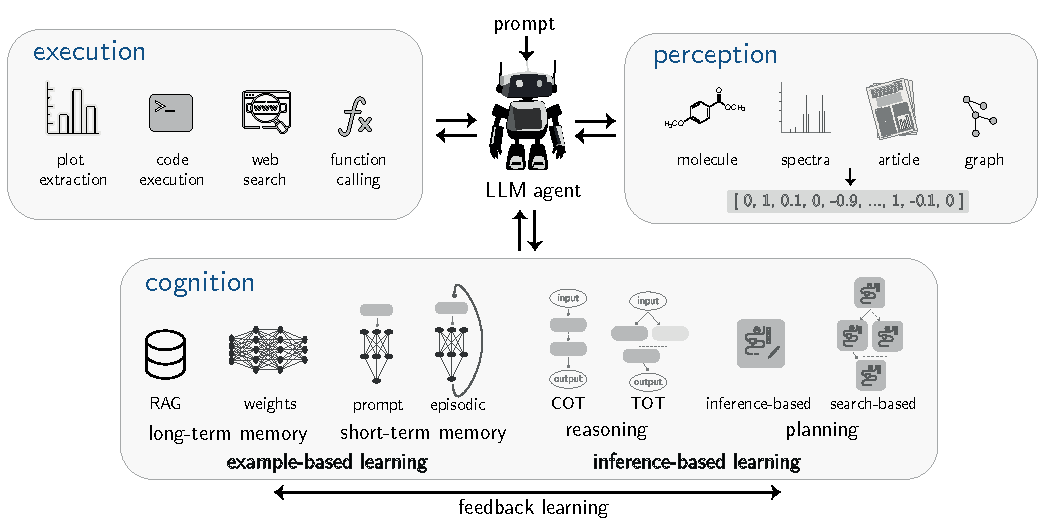
\includegraphics[width=1\textwidth]{figures/rescaled_figures/chemrev_figure7.pdf}
    \caption{\textbf{The execution-cognition-perception capabilities of an \gls{llm}-agent:} This figure illustrates how agents orchestrate complex problems. At the core, an \gls{llm}-agent coordinates multiple capabilities. Upon prompting, the agent can execute tools. Tools include but are not limited to running code, searching for information, or calling functions. These actions feed into the agent's perception system, which transforms raw data into structured representations (in combination, for example, agents can obtain figures' information by executing \gls{ocr} tools on paper). The cognitive architecture underneath serves as the \enquote{agent's brain}, utilizing both memory systems (long-term knowledge storage and short-term contextual awareness) alongside reasoning mechanisms and planning strategies. This creates a dynamic setup, where execution produces observations, cognition interprets those observations and formulates plans, and new actions are taken based on improved understanding.}
    \label{fig:agent-loop}
\end{figure}

\subsubsection{Core Components of an Agentic System}\label{sec:arch_agents}

An agent is a system composed of several key components that work in concert.

\paragraph{Cognitive Engine} This is typically a powerful \gls{llm}. It is responsible for all high-level reasoning, including understanding the user's objective, breaking it down into smaller, manageable steps (see planning \Cref{sec:planning}), and deciding which tools to use to accomplish each step.

\paragraph{Tool Augmentations (Execution)}
\label{sec:tool_augmentation}
Tools are external programs or functions that the agent can call upon to perform actions. They allow agents to interact with the world beyond their internal knowledge. \autocite{schick2023toolformer, parisi2022talm}. Tool augmentation can range from simple tools, such as calculators, to more complex systems that involve web searches, code execution, and integration with robots \autocite{darvish2025organa, chan2024mle, wei2025browsecomp}. In a chemical context, tools can be as simple as a stoichiometry calculator or as complex as a Python script that runs a \gls{dft} simulation using specialized software, a search \gls{api} for querying chemical databases like \modelname{PubChem}, or a controller for a robotic synthesis platform \autocite{boiko2023autonomous, darvish2025organa, bran2024augmenting}.

\paragraph{Memory \& \gls{rag} }
\label{sec:rag}
Agents need to maintain context over long and complex tasks. The memory module provides this capability. Short-term memory is often handled within the finite context window (i.e., number of tokens an \gls{llm} can process), keeping track of the immediate chain of thought and recent actions.
While short-term memory (e.g., context) is transient, \glspl{llm}'s model weights serve as long-term memory. However, these weights often lead to reduced performance on knowledge-intensive scientific tasks and increased susceptibility to hallucinations---generating incorrect or fabricated information \autocite{marcus2020next}.
One effective way to address this limitation is to pair the model with an external knowledge base.\autocite{lewis2020retrieval} Such Long-term memory can be implemented using external databases (e.g., vector stores) where the agent can store and retrieve key findings, successful strategies, or experimental results from past interactions, enabling it to learn and improve over time \autocite{chen2023chemist}. The widely adopted execution of Long-term memory is \gls{rag}. \gls{rag} works by retrieving a set of relevant documents from a designated knowledge database based on the input query. These retrieved documents are then concatenated with the original prompt and passed to the \gls{llm}, which generates the final output.  In scientific applications, this is particularly valuable, as the system can be continuously updated with the latest research and discoveries. In the field of chemistry, \gls{rag} has primarily been used to answer domain-specific questions based on scientific literature and assist in experimental design \autocite{chen2023chemist, skarlinski2024language}.


\subsubsection{Approaches for Building Agentic System}

A well-known approach for building \gls{llm}-based agents is called \gls{react}\autocite{yao2023react}. In \gls{react}, the agent repeatedly goes through a cycle of thinking, performing an action, and then reasoning about the tool output. 
This structured problem-solving is achieved by prompting the model to generate its response following a specific \enquote{Think}, \enquote{Act}, \enquote{Observe} format.
First, the agent considers the problem it needs to solve, focusing on its primary objective. It devises a plan, identifies any missing information, and determines which tool can help it move forward. Next, the agent acts by selecting and utilizing the appropriate tool with the necessary information. For instance, if it needs to find a compound's boiling point, it might use a tool that searches a chemical database using the compound's name or its \gls{smiles} string. After that, the agent observes the outcome by examining the tool's output. This output then becomes new information for the agent. The agent then repeats the cycle, taking this new observation into account as it plans its following action. This loop continues until the agent reaches its main goal. This repeating process helps the agent deal with mistakes, adjust to unexpected results, and break down a big task, like \enquote{finding a better catalyst for this reaction}, into smaller, manageable steps that involve using tools.

While a single agent can effectively tackle linear problems---tasks that can be solved through a predictable sequence of steps---complex scientific discovery often requires diverse expertise and collaborative problem-solving. This has led to the development of multi-agent systems, which move beyond a single cognitive engine to orchestrate a team of agents that work together \autocite{wu2023autogen}. These systems can solve tasks that are too complex or multifaceted for any single agent to handle alone by enabling agents to communicate, delegate, and debate. \autocite{lazaridou2020emergent}
Several collaborative paradigms have emerged, each offering unique advantages:

\paragraph{Specialization and Division of Labor} \label{sec:multi-agent}
Just as a human research group has members with different roles, multi-agent systems can be composed of specialized agents. For example, in a chemistry context, a \enquote{Planner} agent might design a high-level research plan, a \enquote{Literature Searcher} agent could retrieve relevant papers, a \enquote{Computational Chemist} agent could run \gls{dft} simulations, and a \enquote{Safety Expert} agent could check proposed reaction steps for hazards.\autocite{Zou2025ElAgente} This division of labor shows this role-playing approach to be highly effective for complex tasks like software development, where agents take on roles such as \enquote{programmer}, \enquote{tester}, and \enquote{documenter} \autocite{qian2024chatdevcommunicativeagentssoftware}.

\paragraph{Refinement of Answers} A key weakness of single \glspl{llm} is their tendency to hallucinate or pursue a flawed line of reasoning. Multi-agent systems can mitigate this by introducing criticism and debate. In this paradigm, one agent might propose a solution (e.g., a synthetic pathway), while a \enquote{Critic} agent is tasked with finding flaws in the proposal. This adversarial or collaborative process forces the system to refine its ideas, correct errors, and explore alternatives, leading to more robust and reliable outcomes \autocite{liang2024encouragingdivergentthinkinglarge, du2023improving}. 

\paragraph{Context Compression through Parallelism}
A significant operational challenge for any \gls{llm}-based system is the finite context window. 
As a task becomes more complex, the conversational history can grow cluttered with irrelevant details, degrading the model's performance.\autocite{chirkova2025provence0, lee2024long1context} 
Multi-agent systems offer a powerful solution to this problem through a strategy that can be described as context compression. 
By assigning sub-tasks to specialized agents, the system allows each agent to operate in parallel with its own clean, dedicated context window. 
For example, a \enquote{Literature Searcher} agent's context is filled only with search queries and retrieved text, while a \enquote{Computational Chemist} agent's context contains only simulation inputs and results. 
These sub-agents essentially act as filters; they process large amounts of information and then \enquote{compress} their findings into concise summaries or structured data. 
These distilled insights are then passed back to a lead agent or aggregated. 
This not only dramatically speeds up information gathering but also ensures that the primary reasoning process is not diluted by excessive or irrelevant information, leading to higher quality and more reliable outcomes \autocite{Breunig2025HowToFixYourContext}.


\paragraph{Swarm Intelligence and Parallel Exploration}
Inspired by natural systems like ant colonies, some multi-agent approaches use a \enquote{swarm} of less-specialized agents to explore a vast problem space in parallel. Instead of assigning fixed roles, a multitude of agents can independently investigate different hypotheses or search different regions of a chemical space. Their collective findings can then be aggregated to identify the most promising solutions. This is particularly powerful for optimization and discovery tasks, such as high-throughput virtual screening or materials design, where the goal is to efficiently search an enormous number of possibilities \autocite{chen2023agentversefacilitatingmultiagentcollaboration}.


It is also crucial to distinguish between the foundational model itself (e.g., the GPT-4 \gls{llm}) and the \enquote{system} with which the user interacts (e.g., ChatGPT). 
Such systems are not merely the raw model; they incorporate additional layers for safety, prompt management, and some of the adaptation techniques discussed in this section. Understanding this distinction is key to understanding how a static model is transformed into a dynamic and useful tool.